
% v2-acmsmall-sample.tex, dated March 6 2012
% This is a sample file for ACM small trim journals
%
% Compilation using 'acmsmall.cls' - version 1.3 (March 2012), Aptara Inc.
% (c) 2010 Association for Computing Machinery (ACM)
%
% Questions/Suggestions/Feedback should be addressed to => "acmtexsupport@aptaracorp.com".
% Users can also go through the FAQs available on the journal's submission webpage.
%
% Steps to compile: latex, bibtex, latex latex
%
% For tracking purposes => this is v1.3 - March 2012
\documentclass[prodmode,acmtecs]{acmsmall} % Aptara syntax
\usepackage[spanish,polish]{babel}
\usepackage[T1]{fontenc}
\usepackage{fancyvrb}
\usepackage{graphicx,hyperref}
\newcommand\cutout[1]{}


\usepackage[table]{xcolor}
\usepackage[utf8]{inputenc}
\usepackage[parfill]{parskip}
\usepackage{tabulary}
\PassOptionsToPackage{hyphens}{url}
\usepackage{hyperref}    
\usepackage[capitalize]{cleveref}


% Metadata Information
% !!! TODO: SET THESE VALUES !!!
\acmVolume{0}
\acmNumber{0}
\acmArticle{CFP}
\acmYear{0}
\acmMonth{0}

\newcounter{colstart}
\setcounter{page}{4}

\RecustomVerbatimCommand{\VerbatimInput}{VerbatimInput}%
{
%fontsize=\footnotesize,
fontfamily=\rmdefault
}


\newcommand{\UnderscoreCommands}{%\do\verbatiminput%
\do\citeNP \do\citeA \do\citeANP \do\citeN \do\shortcite%
\do\shortciteNP \do\shortciteA \do\shortciteANP \do\shortciteN%
\do\citeyear \do\citeyearNP%
}

\usepackage[strings]{underscore}



% Document starts
\begin{document}


\setcounter{colstart}{\thepage}

\acmArticle{CFP}
\title{\huge\sc SIGLOG Monthly 212}
\author{DAVID PURSER\affil{Max Planck Institute for Software Systems, Saarbr\"ucken}
\vspace*{-2.6cm}\begin{flushright}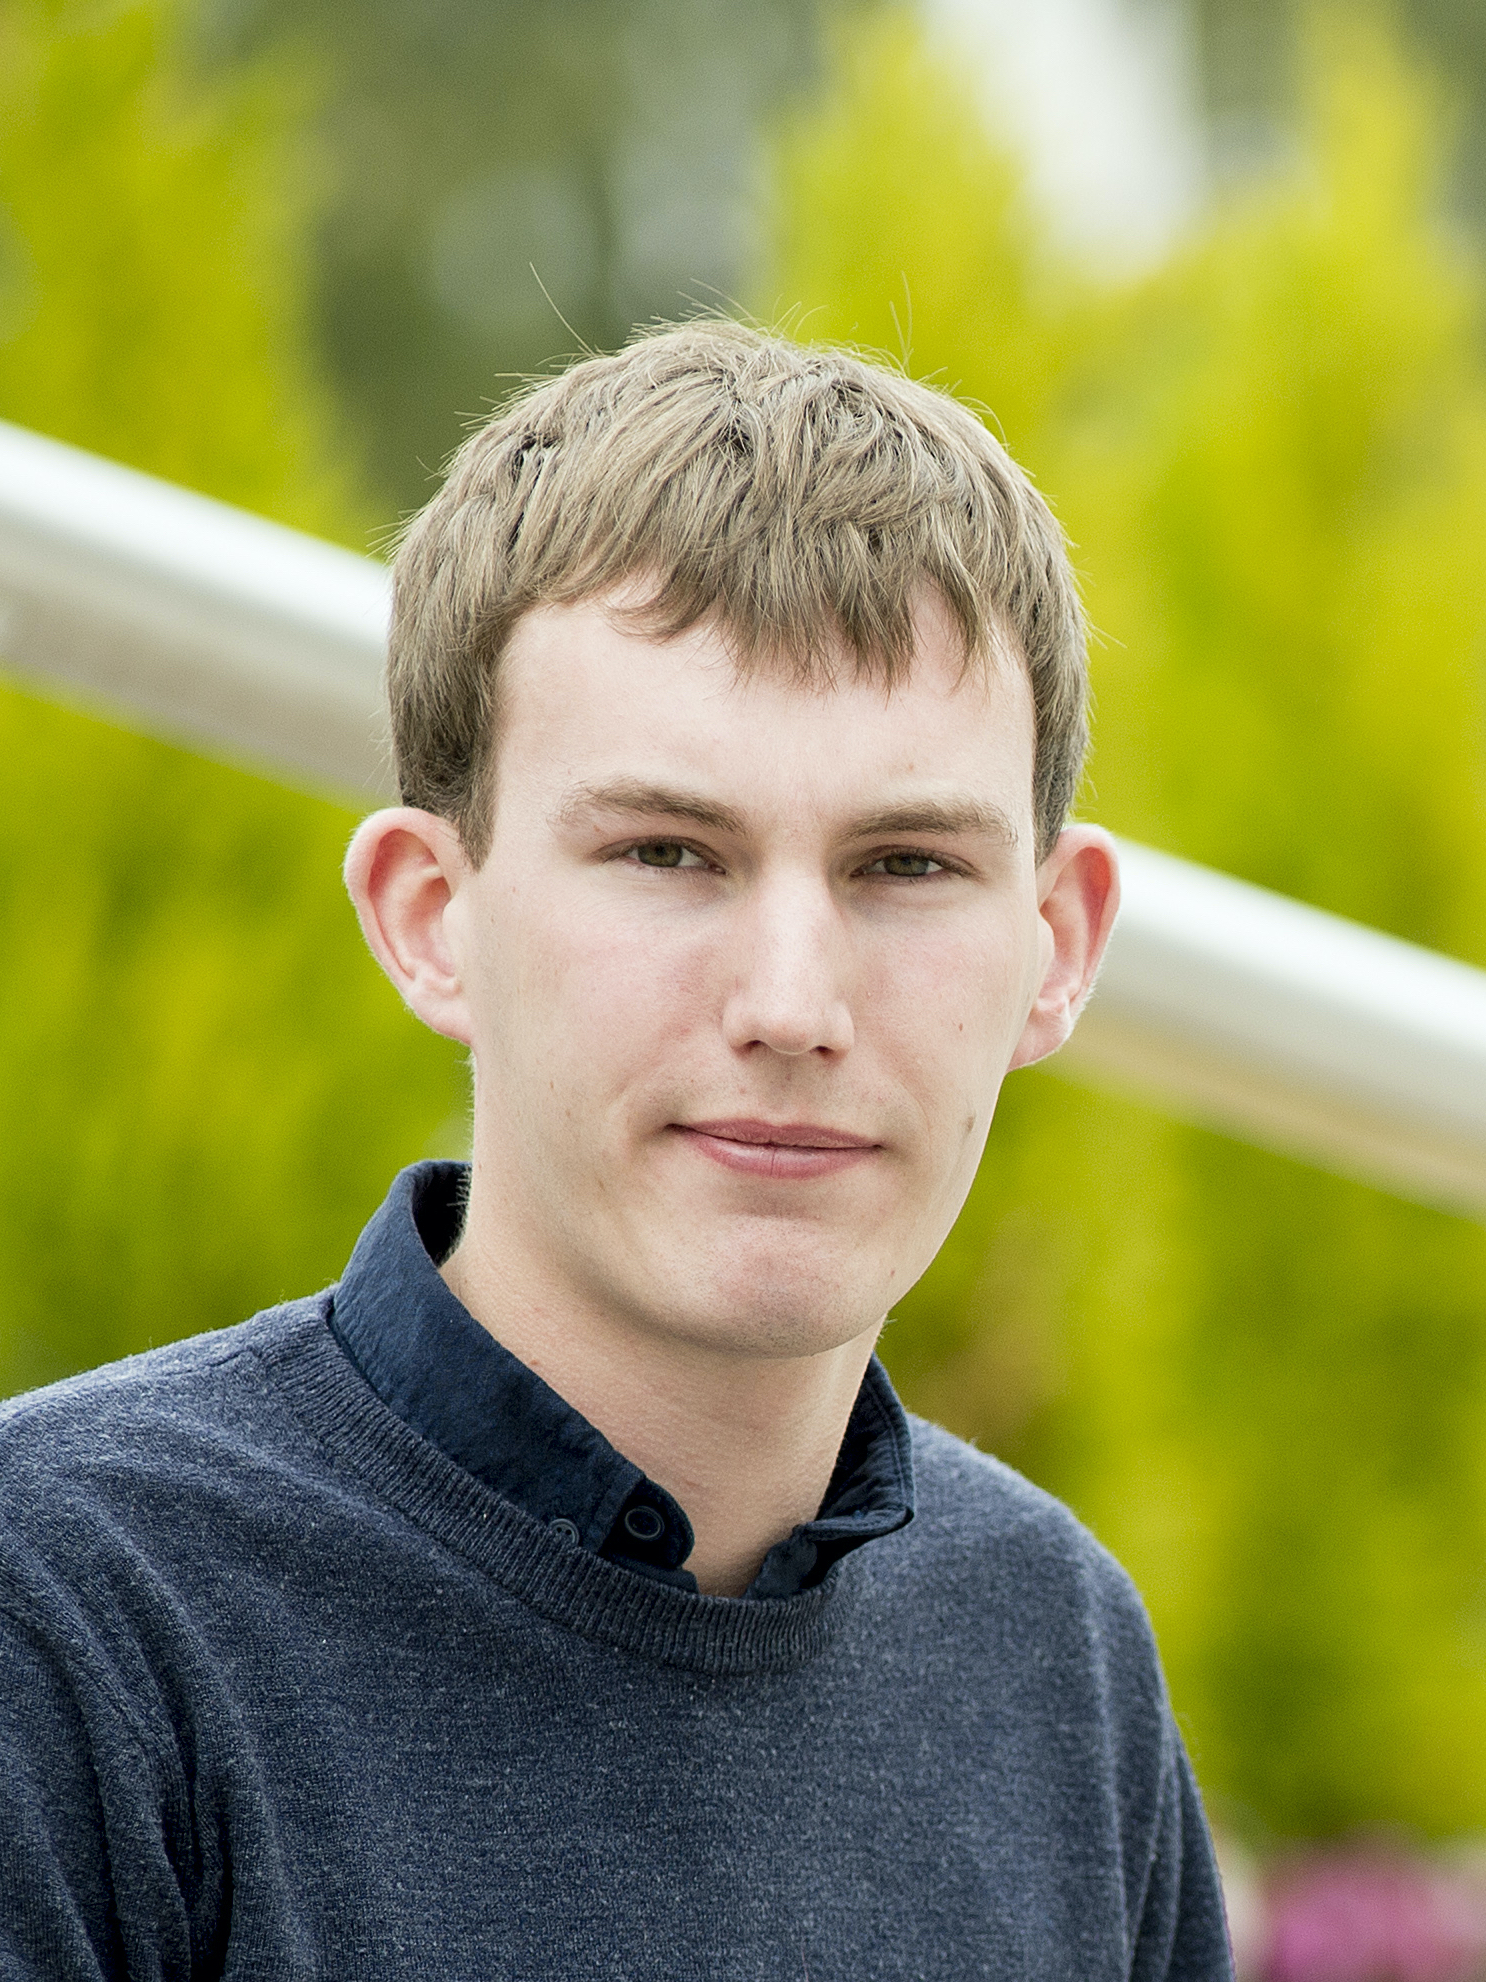
\includegraphics[width=30mm]{dp}\end{flushright}
}

\maketitlee

\href{https://lics.siglog.org/newsletters/}{Past Issues}
 - 
\href{https://lics.siglog.org/newsletters/inst.html}{How to submit an announcement}
\section{Table of Content}\begin{itemize}\item DEADLINES (\cref{deadlines}) 
 
\item CALLS 
 
\begin{itemize}\item WiL 2021 (CALL FOR CONTRIBUTIONS) (\cref{WiL2021})
\item Logic Colloquium 2020 (CALL FOR PAPERS) (\cref{LogicColloquium2020})
\item Tenth Summer School on Formal Techniques (CALL FOR PARTICIPATION) (\cref{TenthSummerSchoolonFormalTechniques})
\item VCLA Awards 2021 (CALL FOR NOMINATIONS) (\cref{VCLAAwards2021})
\item FSEN 2021 (CALL FOR PARTICIPATION) (\cref{FSEN2021})
\item VEST 2021 (CALL FOR TALKS) (\cref{VEST2021})
\item ACM Transactions on Computational Logic (CALL FOR NOMINATIONS) (\cref{ACMTransactionsonComputationalLogic})
\item FCT 2021 (CALL FOR PAPERS) (\cref{FCT2021})
\item RV 2021 (CALL FOR PAPERS) (\cref{RV2021})
\item FedCSIS’2021 (CALL FOR PAPERS) (\cref{FedCSIS2021})
\item CALCO 2021 (CALL FOR PAPERS) (\cref{CALCO2021})
\item EXPRESS/SOS 2021 (CALL FOR PAPERS) (\cref{EXPRESSSOS2021})
\end{itemize} 
\end{itemize}\section{Deadlines}\label{deadlines}\rowcolors{1}{white}{gray!25}\begin{tabulary}{\linewidth}{LL}Alonzo Church Award:  & Apr 01, 2021 (Deadline for Nominations (Extended)) \\
Diagrams 2021:  & Apr 01, 2021 (Titles+short abstracts), Apr 08, 2021 (Long and Short Papers), Apr 15, 2021 (Abstracts and Posters) \\
MGS 21:  & Apr 01, 2021 (Registration deadline) \\
FORMATS 2021:  & Apr 06, 2021 (Abstract), Apr 13, 2021 (Paper) \\
E. W. Beth Outstanding Dissertation Prize 2021:  & Apr 15, 2021 (Deadline for nominations) \\
SPIN 2021:  & Apr 20, 2021 (Paper (extended)) \\
CONCUR 2021:  & Apr 23, 2021 (Abstract), Apr 30, 2021 (Paper) \\
MFCS 2021:  & Apr 30, 2021 (Abstract), May 03, 2021 (Paper) \\
WiL 2021:  & Apr 30, 2021 (Abstract) \\
Logic Colloquium 2020:  & Apr 30, 2021 (Abstract) \\
Tenth Summer School on Formal Techniques:  & Apr 30, 2021 (Guideline registration deadline) \\
VCLA Awards 2021:  & Apr 30, 2021 (Submission deadline) \\
FSEN 2021:  & May 01, 2021 (Registration deadline) \\
VEST 2021:  & May 03, 2021 (Talk) \\
ACM Transactions on Computational Logic:  & May 07, 2021 (Nominations for Editor-In-Chief) \\
FCT 2021:  & May 09, 2021 (Abstract), May 16, 2021 (Paper) \\
RV 2021:  & May 13, 2021 (Abstract), May 20, 2021 (Paper) \\
FedCSIS’2021:  & May 24, 2021 (Paper) \\
ICGI 2020/21:  & May 25, 2021 (Paper) \\
CALCO 2021:  & Jun 03, 2021 (Paper) \\
EXPRESS/SOS 2021:  & Jun 21, 2021 (Paper) \\
ACKERMANN AWARD 2021:  & Jul 01, 2021 (Deadline for nomination) \\
CSL22:  & Jul 05, 2021 (Abstract), Jul 12, 2021 (Paper) \\
\end{tabulary}
\section{WiL 2021: 5th Women in Logic Workshop}\label{WiL2021}  June 27, 2021 part of LICS 2021\\ 
  \href{https://sites.google.com/g.uporto.pt/wil2021}{https://sites.google.com/g.uporto.pt/wil2021}\\ 
CALL FOR CONTRIBUTIONS 

\begin{itemize}\item  Women in Logic 2021 is a satellite event of the 36th Annual ACM/IEEE  Symposium on Logic in Computer Science (LICS’21) to be held virtually  on June 29-July 2, 2021. 
 
  The Women in Logic workshop (WiL) provides an opportunity to increase awareness of the valuable contributions made by women in the area of logic in computer science. Its main purpose is to promote the excellent research done by women, with the ultimate goal of increasing their visibility and representation in the community. Our aim is to: 
 
\begin{itemize}\item  provide a platform for female researchers to share their work and achievements;
\item  increase the feelings of community and belonging, especially among junior faculty, post-docs and students through positive interactions with peers and more established faculty;
\item  establish new connections and collaborations;
\item  foster a welcoming culture of mutual support and growth within the logic research community. We believe these aspects will benefit women working in logic and computer science, particularly early-career researchers.
\end{itemize} 
  Previous versions of Women in Logic (Reykjavík, Iceland 2017, Oxford, UK 2018, Vancouver, Canada 2019, and Paris, France 2020)  were very successful in showcasing women's work and as catalysts for a  recognition of the need for change in the community. 
 
\item  TOPICS 
 
  Topics of interest include but are not limited to:  
 
  automata theory, automated deduction, categorical models and logics, concurrency and distributed computation, constraint programming, constructive mathematics, database theory, decision procedures, description logics, domain theory, finite model theory, formal aspects of program analysis, formal methods, foundations of computability, games and logic, higher-order logic, lambda and combinatory calculi, linear logic, logic in artificial intelligence, logic programming, logical aspects of bioinformatics, logical aspects of computational complexity, logical aspects of quantum computation, logical frameworks, logics of programs, modal and temporal logics, model checking, probabilistic systems, process calculi, programming language semantics, proof theory, real-time systems, reasoning about security and privacy, rewriting, type systems and type theory, and verification. 
 
\item INVITED SPEAKERS 
 
  Simona Ronchi Della Rocca and Rineke Verbrugge 
 
\item  IMPORTANT DATES 
 
\rowcolors{1}{white}{gray!25}\begin{tabulary}{\linewidth}{LL}Abstract submission:  & Apr 30, 2021 \\
Notification:  & May 28, 2021 \\
Workshop:  & Jun 27, 2021 \\
\end{tabulary}
 
\item  SUBMISSIONS 
 
  Abstracts should be written in English (1-2 pages), and prepared using the Easychair style (\href{https://easychair.org/publications/for_authors}{https://easychair.org/publications/for\_authors}) and submitted as a PDF to \href{https://easychair.org/conferences/?conf=wil2021}{https://easychair.org/conferences/?conf=wil2021} 
 
\end{itemize}\section{Logic Colloquium 2020:}\label{LogicColloquium2020}  July 19-24, 2020, Poznań, Poland (online)\\ 
  NO FEES APPLY\\ 
  \href{https://lc2021.pl/}{https://lc2021.pl/}\\ 
CALL FOR PAPERS 

\begin{itemize}\item  The Logic Colloquium is the European Summer Meeting of the Association for Symbolic Logic, that in 2021 will be hosted from 19th to 24th of July by the Adam Mickiewicz University, Poznań, Poland, as a fully on-line event. It is organized jointly by the AMU Faculties: of Psychology and Cognitive Science and of Mathematics and Computer Science. 
 
  \href{https://easychair.org/conferences/?conf=lc20210}{https://easychair.org/conferences/?conf=lc20210} 
 
\item  DATES: 
 
\rowcolors{1}{white}{gray!25}\begin{tabulary}{\linewidth}{LL}Registration open:  & Mar 31, 2021 \\
Abstract submission:  & Apr 30, 2021 \\
Notification:  & May 20, 2021 \\
Camera-ready abstracts due:  & Jun 01, 2021 \\
\end{tabulary}
 
\item  Detailed information can be found on the webpage. 
 
\end{itemize}\section{Tenth Summer School on Formal Techniques:}\label{TenthSummerSchoolonFormalTechniques} May 22 - May 28, 2021, Online (Postponed from 2020)\\ 
 \href{http://fm.csl.sri.com/SSFT21}{http://fm.csl.sri.com/SSFT21}\\ 
CALL FOR PARTICIPATION 

\begin{itemize}\item  Techniques based on formal logic, such as model checking, satisfiability, static analysis, and automated theorem proving, are finding a broad range of applications in modeling, analysis, verification, and synthesis. This school, the tenth in the series, will focus on the principles and practice of formal techniques, with a strong emphasis on the hands-on use and development of this technology. It primarily targets graduate students and young researchers who are interested in studying and using formal techniques in their research. A prior background in formal methods is helpful but not required. Participants at the school can expect to have a seriously fun time experimenting with the tools and techniques presented in the lectures during laboratory sessions. 
 
\item  The lecturers at  the school include: 
 
\begin{itemize}\item  Thomas Reps (University of Wisconsin), Algebraic Program Analysis: Automating Abstract Interpretation
\item  Natasha Sharygina (University of Lugano, Switzerland), SMT-streamlined Software Model Checking
\item  Warren A. Hunt, Jr. and J Strother Moore (University of Texas), Proving Properties of Algorithms, Hardware, and Software with ACL2
\item  Jose Meseguer (University of Illinois at Urbana-Champaign), Executable Formal Specification and Verification in Maude
\end{itemize} 
\item  The main lectures in the summer school start on Monday May 24 and will be preceded by a background course on logic on Saturday May 22 and Sunday May 23: 
 
\begin{itemize}\item  Natarajan Shankar (SRI CSL) and Stephane Graham-Lengrand (Ecole Polytechnique) Speaking Logic
\end{itemize} 
\item  The summer school also include several distinguished invited talks.  
 
\item  REGISTRATION 
 
  \href{http://fm.csl.sri.com/SSFT21}{http://fm.csl.sri.com/SSFT21} 
 
  Those who already registered for the 2020 event need not re-register, and you will be contacted to check if you would like your registration to be processed. Although the summer school is virtual and there is no registration fee, attendance is restricted to registered participants. Attendees who complete the summer school will receive a certificate by mail.  
 
  Applications should be submitted together with names of two references (preferably advisors, professors, or senior colleagues).   
 
  Applicants are urged to submit their applications before April 30, 2021, since there are only a limited number of spaces available.  
 
  We strongly encourage the participation of women and under-represented minorities in the summer school. 
 
\end{itemize}\section{VCLA Awards 2021: The Vienna Center for Logic and Algorithms of TU Wien Awards for Outstanding Theses and Scientific Works}\label{VCLAAwards2021}  \href{https://logic-cs.at/vcla-international-student-awards-2021}{https://logic-cs.at/vcla-international-student-awards-2021}\\ 
CALL FOR NOMINATIONS 

\begin{itemize}\item  The Vienna Center for Logic and Algorithms of TU Wien (Vienna University of Technology), calls for the nomination of authors of outstanding theses and scientific works in the field of Logic and Computer Science, in the following two categories: 
 
\begin{itemize}\item The Outstanding Master Thesis Award:  1200 EUR
\item The Outstanding Undergraduate Thesis Award: 800 EUR (Bachelor thesis or equivalent, 1st cycle of the Bologna process)
\end{itemize} 
  The winners will be invited to present their work at an award ceremony in Vienna, if the situation allows 
 
\item  The main areas of interest are: 
 
\begin{itemize}\item Computational Logic, covering theoretical and mathematical foundations such as proof theory, model theory, computability theory, Boolean satisfiability (SAT), QBF, constraint satisfaction, satisfiability modulo theories, automated deduction (resolution, refutation, theorem proving), non-classical logics (substructural logics, multi-valued logics, deontic logics, modal and temporal logics).
\item Algorithms and Computational Complexity, including design and analysis of discrete algorithms, complexity analysis, algorithmic lower bounds, parameterized and exact algorithms, decomposition methods, approximation algorithms, randomized algorithms, algorithm engineering, as well as algorithmic game theory, computational social choice, parallel algorithms, graph drawing algorithms, and distributed algorithms.
\item Databases and Artificial Intelligence, concerned with logical methods for modeling, storing, and drawing inferences from data and knowledge. This includes subjects like query languages based on logical concepts (Datalog, variants of SQL, XML, and SPARQL), novel database-theoretical methods (schema mappings, information extraction and integration), logic programming, knowledge representation and reasoning (ontologies, answer-set programming, belief change, inconsistency handling, argumentation, planning).
\item Verification, concerned with logical methods and automated tools for reasoning about the behavior and correctness of complex state-based systems such as software and hardware designs as well as hybrid systems. This ranges from model checking, program analysis and abstraction to new interdisciplinary areas such as fault localization, program repair, program synthesis, and the analysis of biological systems.
\end{itemize} 
\item  ELIGIBILITY 
 
\begin{itemize}\item  The degree must have been awarded between November 15th, 2019 and December 31st, 2020 (inclusive)
\item Submissions already submitted to the VCLA Awards 2020 cannot be re-submitted.
\item Students who obtained their degree at TU Wien are not eligible.
\end{itemize} 
\item  NOMINATION REQUIREMENTS 
 
  Nominations must include: 
 
\begin{itemize}\item  A cover page that contains the name and contact details of the nominated person, the title of the work for which the person is being nominated, award category, the date on which the degree was awarded, and the name of the university
\item  An English summary of the thesis of maximum 3 pages, excluding references (A4 or letter page size, 11pt font min). The summary must clearly state the main contribution of the work, its novelty, and its relevance to some of the aforementioned areas of interest
\item  The CV of the nominated person, including publication list (if applicable)
\item  An endorsement letter from a supervisor or another proposing person. The letter must clearly state the independent and novel contribution of the student, and why the proposer believes the student deserves the award. 
\item  The full thesis
\end{itemize} 
  All documents should be in English, with the exception of the thesis. In case the thesis is in a different language, it must be accompanied by a research report in English of at least 10 pages that should be sufficient for the committee to evaluate the merit and quality of the submitted work.  
 
\item  INSTRUCTIONS FOR SUBMITTING SELF-NOMINATIONS 
 
\begin{itemize}\item  Nominations should be submitted electronically by the applicants: \href{https://easychair.org/conferences/?conf=vclaawards2021}{https://easychair.org/conferences/?conf=vclaawards2021}
\item  Submissions consist of two pdf files. The first is a single pdf file containing all documents for the nomination except the full thesis; the documents should appear in the order they are listed above. The second pdf file is the full thesis
\item  The endorsement letter may be provided after the submission deadline, and  may optionally be sent by email by the endorser and omitted from the Easychair submission. In this case, please email the letter as a pdf file, including the name of the nominated person in the subject, to award (AT) logic-cs (DOT) at.
\item  The submission must be accompanied by a plain text electronic abstract of the thesis of at most 400 words, and three keywords. 
\item   The nominated student must be listed as the only author in the submission form.
\end{itemize} 
\item  IMPORTANT DATES (AoE) 
 
\rowcolors{1}{white}{gray!25}\begin{tabulary}{\linewidth}{LL}Submission deadline:  & Apr 30, 2021 \\
Notification of decision:  & After Jul 15, 2021 \\
Award ceremony:  & Depending on the COVID-19 situation \\
\end{tabulary}
 
\item  CONTACT: award (AT) logic-cs (DOT) at 
 
\end{itemize}\section{FSEN 2021: Ninth International Conference on Fundamentals of Software Engineering 2021 Theory and Practice}\label{FSEN2021}  \href{http://fsen.ir/2021/}{http://fsen.ir/2021/}\\ 
  19 - 21 May, 2021, Virtual Conference\\ 
CALL FOR PARTICIPATION 

\begin{itemize}\item  FSEN is an international conference that aims to bring together researchers, engineers, developers, and practitioners from the academia and the industry to present and discuss their research work in the area of formal methods for software engineering. 
 
\item  FSEN 2021 will be held online from Wednesday, May 19th to Friday, May 21st, 2021. The three-day event includes three keynote talks and seven sessions as well as a number of social events in the form of a virtual tour along the many beautiful and historical places in Iran. The preliminary conference programme can be found at: \href{http://www.fsen.ir/2021/Programme.aspx}{http://www.fsen.ir/2021/Programme.aspx} 
 
\item  REGISTRATION  
 
  Attendance is free of charge but requires registration.  
 
Registration deadline: May 01, 2021 
 
  \href{http://www.fsen.ir/2021/Registration.aspx}{http://www.fsen.ir/2021/Registration.aspx} 
 
\item  KEYNOTE SPEAKERS 
 
\begin{itemize}\item  Marta Kwiatkowska, University of Oxford
\item  Mira Mezini, Technische Universität Darmstadt
\item  Pavol Cerny, Vienna University of Technology 
\end{itemize} 
\end{itemize}\section{VEST 2021: 2nd Workshop on Verification of Session Types}\label{VEST2021}  Online on July 12, 2021, co-located with ICALP 2021\\ 
  \href{https://sites.google.com/view/vest21/home}{https://sites.google.com/view/vest21/home}\\ 
CALL FOR TALKS 

\begin{itemize}\item  PRESENTATION 
 
  The goal of this workshop is to bring together researchers and build and strengthen a community working on verification of session types using various theorem provers such as Agda, Coq, Isabelle or any other. 
 
  Session types are abstract representations of the sequences of operations that computational entities (such as channels or objects) must perform. Stateful entities offer services in a non-uniform way (one cannot pop from an empty stack); traditional type systems cannot guarantee that operations are only invoked when the entity is in the right state. 
 
  Large-scale software systems rely on message-passing protocols: their correctness largely depends on sound protocol implementations. Session types can help in the specification of correct-by-construction systems, and in verifying that programs respect their intended protocols. 
 
  Recent years have seen a steady stream of research on behavioural types: their foundations and their transfer to several programming languages. This has led to highly-cited papers in conferences such as POPL and journals such as TOPLAS. Research projects on behavioural types have advanced the theory and applications of behavioural types. 
 
  Although the foundations of session types are now well established, and new works build on approaches that have become standard, there is still a lack of reusable libraries, namely machine-verified ones. As on one hand the basis of most works is common, and on the other hand the complexity of the formal systems is considerable and may lead to errors in the proofs of the soundness results, machine verifying the type systems proposed is vital. Libraries, or at least clear formalisations of common approaches, is crucial to avoid not only to repeat work but also to increase the confidence in the knowledge base. Moreover, as many of these systems have a goal to do static analysis to ensure some safety or liveness property, machine verification of these approaches leads to certified software for program analysis. 
 
  The goal of the VEST workshop is to gather the researchers working on mechanisations of behavioural types using various theorem provers, such as Agda, Coq, Isabelle or any other. The workshop will be a platform to present both the now well-established efforts and the ongoing works the community has put on verification. The workshop will also be a forum to discuss strengths and weaknesses of existing approaches, potential obstacles and to foster collaboration. 
 
\item  TYPES OF CONTRIBUTIONS 
 
  We request two types of research contributions.  
 
\begin{itemize}\item  Type 1: Short presentations (1 page) of work published elsewhere;
\item  Type 2: Presentations (2-5 pages) of ongoing original work.
\end{itemize} 
  Submissions of Type 1 will consist of 1 page papers presenting the work, the publication venue and the significance of the results; the PC will select the submissions with a ranking system.  
 
  Submissions of Type 2 will consist of 2 - 5 page papers submitted to a light reviewing process. 
 
  There will be no proceedings of VEST'21, but rather the aim is to strengthen and further expand our community. 
 
  Submission Link: \href{https://easychair.org/conferences/?conf=vest21}{https://easychair.org/conferences/?conf=vest21} 
 
\item  Important Dates AoE (UTC-12h) 
 
\rowcolors{1}{white}{gray!25}\begin{tabulary}{\linewidth}{LL}Talk submission:  & May 03, 2021 \\
Notification:  & Jun 14, 2021 \\
Final version:  & Jul 05, 2021 \\
Workshop:  & Jul 12, 2021 \\
\end{tabulary}
 
\end{itemize}\section{ACM Transactions on Computational Logic:}\label{ACMTransactionsonComputationalLogic}  Editor-In-Chief\\ 
CALL FOR NOMINATIONS 

\begin{itemize}\item  The term of the current Editor-in-Chief (EiC) of the ACM Transactions on Computational Logic (TOCL \href{http://tocl.acm.org/}{http://tocl.acm.org/}) is coming to an end, and the ACM Publications Board has set up a nominating committee to assist the Board in selecting the next EiC. 
 
  Nominations, including self-nominations, are invited for a three-year term as TOCL EiC, beginning on July 1, 2021.  The EiC appointment may be renewed at most one time. This is an entirely voluntary position, but ACM will provide appropriate administrative support. 
 
\end{itemize}\begin{itemize}\item  Appointed by the ACM Publications Board, Editors-in-Chief (EiCs) of ACM journals are delegated full responsibility for the editorial management of the journal consistent with the journal's charter and general ACM policies. The Board relies on EiCs to ensure that the content of the journal is of high quality and that the editorial review process is both timely and fair. He/she has the final say on acceptance of papers, size of the Editorial Board, and appointment of Associate Editors. A complete list of responsibilities is found in the ACM Volunteer Editors Position Descriptions (\href{http://www.acm.org/publications/policies/position_descriptions}{http://www.acm.org/publications/policies/position\_descriptions}). Additional information can be found in the following documents: 
 
\begin{itemize}\item  Roles and Responsibilities in ACM Publishing 
\end{itemize} 
    \href{https://www.acm.org/publications/policies/roles-and-responsibilities}{https://www.acm.org/publications/policies/roles-and-responsibilities} 
 
\begin{itemize}\item  ACM's Evaluation Criteria for Editors-in-Chief
\end{itemize} 
    \href{http://www.acm.org/publications/policies/evaluation/}{http://www.acm.org/publications/policies/evaluation/} 
 
  Nominations should include a vita along with a brief statement of why the nominee should be considered. Self-nominations are encouraged and should include a statement of the candidate's vision for the future development of TOCL. The deadline for submitting nominations is May 7, 2021, although nominations will continue to be accepted until the position is filled.  
 
\item  Please send all nominations to the search committee chair, Dale Miller (dale.miller@inria.fr).  
 
  The search committee members are: 
 
\begin{itemize}\item  Dale Miller (Inria \& LIX/IPP, France), Chair
\item  Christel Baier (TU Dresden, Germany)
\item  Prakash Panangaden (McGill University, Canada)
\item  Andrew Pitts (University of Cambridge, UK)
\item  Simona Ronchi Della Rocca (University of Turin, Italy)
\item  Adelinde Uhrmacher (University of Rostock, Germany) ACM Pubs Board Liaison
\end{itemize} 
\end{itemize}\section{FCT 2021: 23rd International Symposium on Fundamentals of Computation Theory}\label{FCT2021}  September 12-15, 2021, Athens, Greece\\ 
  \href{https://www.corelab.ntua.gr/fct2021}{https://www.corelab.ntua.gr/fct2021}\\ 
  Submission deadline: May 16, 2021\\ 
CALL FOR PAPERS 

\begin{itemize}\item  ABOUT FCT 
 
  The Symposium on Fundamentals of Computation Theory (FCT) was established in 1977 as a forum for researchers interested in all aspects of theoretical computer science, and in particular algorithms, complexity, formal and logical methods. FCT is a biennial series of conferences, previously held in Poland, Germany, Hungary, Sweden, Russia, Romania, Latvia, Norway, United Kingdom, France, and Denmark. The last five Symposia were held in Oslo (2011), Liverpool (2013), Gdansk (2015), Bordeaux (2017), and Copenhagen (2019). 
 
  FCT 2021 will be hosted by the National Technical University of Athens partially or completely online, depending on the status of the COVID-19 pandemic. 
 
\item  IMPORTANT DATES 
 
\rowcolors{1}{white}{gray!25}\begin{tabulary}{\linewidth}{LL}Abstract submission:  & May 9, 2021 (AoE) \\
Paper submission:  & May 16, 2021 (AoE) \\
Notification to authors:  & Jun 28, 2021 \\
Camera-ready submission:  & Jul 06, 2021 \\
Symposium:  & Sep 12-15, 2021 \\
\end{tabulary}
 
\item  SCOPE 
 
  The program committee is soliciting original and significant research contributions to the fundamentals of computation theory, including (but not limited to): 
 
\begin{itemize}\item  Algorithms: algorithm design and optimization, data structures, combinatorics and analysis of algorithms, randomized algorithms, approximation algorithms, parameterized and exact algorithms, computational algebra and number theory, computational geometry, parallel algorithms, distributed algorithms and protocols, online algorithms, streaming algorithms, algorithmic game theory, computational foundations of machine learning, computational biology 
\item  Complexity: models of computation, computational complexity, decidability, Boolean/algebraic circuits and functions, randomized computation, derandomization, interactive proofs, computational foundations of cryptography, quantum computation, complexity theory, lower bounds, counting complexity
\item  Formal methods: algebraic and categorical methods, automata and formal languages, database theory, foundations of concurrency and distributed systems, logic and model checking, models of reactive, hybrid, and stochastic systems, principles of programming languages, program analysis and transformation, security, specification, refinement, and verification, type systems, ad hoc, dynamic, and evolving systems, foundations of cloud computing and ubiquitous systems
\end{itemize} 
\item  INVITED SPEAKERS 
 
\begin{itemize}\item  Constantinos Daskalakis, Massachusetts Institute of Technology
\item  Claire Mathieu, CNRS and University of Paris
\item  Nobuko Yoshida, Imperial College London
\end{itemize} 
\item  PROCEEDINGS 
 
  Conference proceedings will be published in the ARCoSS subline of the Springer ``Lecture Notes in Computer Science'' series. 
 
\item  Special Issue 
 
  Selected papers will be invited to a special issue of the ``Journal of Computer and System Sciences'', devoted to FCT 2021. 
 
\item  AWARDS 
 
  Awards will be given to the best paper and the best student paper. To be eligible for the best student paper award, at least one of the paper authors must be a full-time student at the time of submission, and the student(s) must have made a significant contribution to the paper. 
 
\item  SUBMISSION 
 
  Authors are invited to submit high-quality manuscripts reporting original  research in the topics related to the symposium.  
 
  Manuscripts must be unpublished, not under simultaneous submission to venues with proceedings and accepted papers require one author to present. 
 
  Max 12 pages (excluding references), LNCS Template, plus an optional, clearly marked appendix of reasonable length (to be read at the program committee's discretion). The first page must include an indication of whether the paper is eligible for the best student paper award. 
 
  \href{https://easychair.org/conferences/?conf=fct2021}{https://easychair.org/conferences/?conf=fct2021} 
 
\end{itemize}\section{RV 2021: 21st INTERNATIONAL CONFERENCE ON RUNTIME VERIFICATION}\label{RV2021}  Oct 11-14, 2021, Los Angeles, California, US or Online\\ 
  \href{https://www.cs.bgu.ac.il/}{https://www.cs.bgu.ac.il/}~rv21/\\ 
CALL FOR PAPERS 

\begin{itemize}\item  Runtime verification is concerned with the monitoring and analysis of the runtime behaviour of software and hardware systems. Runtime verification techniques are crucial for system correctness, reliability, and robustness; they provide an additional level of rigor and effectiveness compared to conventional testing and are generally more practical than exhaustive formal verification. Runtime verification can be used prior to deployment, for testing, verification, and debugging purposes, and after deployment for ensuring reliability, safety, and security and for providing fault containment and recovery as well as online system repair. 
 
\item  TOPICS 
 
  Topics of interest include (but are not limited to): specification languages for monitoring, monitor construction techniques, logging, recording, and replay, combination of static and dynamic analysis, specification mining and machine learning over runtime traces, runtime checking of privacy and security policies, metrics and statistical information gathering, program/system execution visualization, fault localization, containment, recovery and repair, dynamic type checking and assurance cases.  
 
\item  IMPORTANT DATES:   
 
\rowcolors{1}{white}{gray!25}\begin{tabulary}{\linewidth}{LL}Abstract submission:  & May 13, 2021 \\
Paper submission:  & May 20, 2021 \\
Author notification:  & Jul 12, 2021 \\
Camera-ready version:  & Aug 02, 2021 \\
\end{tabulary}
 
\item  Detailed information can be found on the webpage. 
 
\end{itemize}\section{FedCSIS’2021: 16th Conference on Computer Science and Intelligence Systems}\label{FedCSIS2021}  Online, 2-5 September, 2021 \\ 
  \href{http://fedcsis.org}{http://fedcsis.org}\\ 
  \href{http://easychair.org/conferences/?conf=fedcsis2021}{http://easychair.org/conferences/?conf=fedcsis2021}\\ 
CALL FOR PAPERS 

\begin{itemize}\item  CONFERENCE 
 
  FedCSIS is an annual international conference, this year organized jointly by the Polish Information Processing Society (PTI), IEEE Poland Section Computer Society Chapter and Bulgarian Academy of Sciences. It is technically sponsored by a number of IEEE units and other professional organizations (for the full list, see the conference site). The mission of the FedCSIS Conference Series is to provide a highly acclaimed forum in computer science and intelligence systems. We invite researchers from around the world to contribute their research results and participate in Technical Sessions, focused on their scientific and professional interests in computer science and intelligence systems. 
 
  Information about FedCSIS indexing / bibliometry / rankings can be found at: \href{https://www.fedcsis.org/2021/indexation}{https://www.fedcsis.org/2021/indexation} 
 
  The FedCSIS 2021 consists of five conference Tracks, hosting Technical Sessions:  
 
\item  Track 1: 
 
  Advanced Artificial Intelligence in Applications (16th Symposium AAIA'21) 
 
\begin{itemize}\item  Computational Optimization (14th Workshop WCO'21)
\end{itemize} 
\item  Track 2: 
 
  Computer Science \& Systems (CSS'21) 
 
\begin{itemize}\item  Actors, Agents, Assistants, Avatars (1st Workshop 4A'21)
\item  Computer Aspects of Numerical Algorithms (14th Workshop CANA'21)
\item  Multimedia Applications and Processing (14th International Symposium MMAP'21)
\item  Scalable Computing (12th Workshop WSC'21)
\end{itemize} 
\item  Track 3: 
 
  Network Systems and Applications (NSA'21) 
 
\begin{itemize}\item  Internet of Things - Enablers, Challenges and Applications (5th Workshop IoT-ECAW'21)
\item  Cyber Security, Privacy and Trust (2nd International Forum NEMESIS'21)
\end{itemize} 
\item  Track 4: 
 
  Advances in Information Systems and Technologies (AIST'21) 
 
\begin{itemize}\item  Data Science in Health, Ecology and Commerce (3rd Special Session DSH'21)
\item  Information Systems Management (16th Conference ISM'21)
\item  Knowledge Acquisition and Management (27th Conference KAM'21)
\end{itemize} 
\item  Track 5: 
 
  Software, System and Service Engineering (S3E'21) 
 
\begin{itemize}\item  Cyber-Physical Systems (8th Workshop IWCPS-8)
\item  Software Engineering (41th IEEE Workshop SEW-41)
\item  Advances in Programming Languages (8th Workshop WAPL'21)
\end{itemize} 
\item  Recent Advances in Information Technology (7th Doctoral Symposium DS–RAIT'21) 
 
\item  KEYNOTE SPEAKERS 
 
  David Bader, Rajkumar Buyya, Hristo Djidjev and Moshe Y. Vardi 
 
\item  PAPER SUBMISSION AND PUBLICATION 
 
\begin{itemize}\item  Papers should be submitted by May 24, 2021 (strict deadline, no extensions): \href{https://easychair.org/conferences/?conf=fedcsis2021}{https://easychair.org/conferences/?conf=fedcsis2021}
\item  Preprints will be published online.
\item  Most Technical Session organizers arrange quality journals, edited volumes, etc., and may invite selected extended and revised papers for post-conference publications (information can be found at the websites of individual events, or by contacting Chairs of said events).
\end{itemize} 
\item  IMPORTANT DATES 
 
\rowcolors{1}{white}{gray!25}\begin{tabulary}{\linewidth}{LL}Paper submission:  & May 24, 2021 (AoE, no extensions) \\
Position paper submission:  & Jun 14, 2021 \\
Author notification:  & Jul 05, 2021 \\
Final paper submission and registration:  & Jul 26, 2021 \\
Conference date:  & Sep 2-5, 2021 \\
\end{tabulary}
 
\end{itemize}\section{CALCO 2021: 9th International Conference on Algebra and Coalgebra in Computer Science }\label{CALCO2021}  31 Aug - 03 Sep 2021  \\ 
  Salzburg, Austria (if possible) \\ 
  Co-located with MFPS XXXV \\ 
  \href{https://www.coalg.org/calco-mfps2021/}{https://www.coalg.org/calco-mfps2021/}\\ 
CALL FOR PAPERS 

\begin{itemize}\item  SCOPE  
 
  Algebraic and coalgebraic methods and tools are a mainstay of computer science. From data types to development techniques and specification formalisms, both theoreticians and practitioners have benefited from the large body of research proposed and implemented since the pioneering works of the 1960s.  
 
  CALCO aims to bring together researchers with interests in both foundational and applicative uses of algebra and coalgebra in computer science, traditional as well as emerging ones  
 
  CALCO is a high-level, bi-annual conference formed by joining the forces and reputations of CMCS (the International Workshop on Coalgebraic Methods in Computer Science) and WADT (the Workshop on Algebraic Development Techniques). Previous CALCO editions took place in Swansea (Wales, 2005), Bergen (Norway, 2007), Udine (Italy, 2009), Winchester (UK, 2011), Warsaw (Poland, 2013), Nijmegen (the Netherlands, 2015), Ljubljana (Slovenia,2017), and London (UK, 2019).  
 
  The 9th edition will be held in Salzburg, Austria, colocated with MFPS XXXVII.  
 
\item  TOPICS OF INTERESTS  
 
  All topics relating to algebraic and coalgebraic theory and applications are of interest for CALCO, and among them  
 
\begin{itemize}\item  Models and logics: Automata and languages, Graph transformations and term rewriting, Modal logics, Proof systems, Relational systems 
\item  Algebraic and coalgebraic semantics: Abstract data types, Re-engineering techniques (program transformation), Semantics of conceptual modelling methods and techniques, Semantics of programming languages 
\item  Methodologies in software and systems engineering: Development processes, Method integration, Usage guidelines 
\item  Specialised models and calculi: Hybrid, probabilistic, and timed systems, Concurrent, distributed, mobile, cyber-physical, and context-aware computational paradigms, Systems theory and computational models (chemical, biological, etc.) 
\item  System specification and verification: Formal testing and quality assurance, Generative programming and model-driven development, Integration of formal specification techniques, Model-driven development, Specification languages, methods, and environments 
\item  Tools supporting algebraic and coalgebraic methods for: Advances in automated verification, Model checking, Theorem proving, Testing 
\item  String diagrams and network theory: Theory of PROPs and operads, Rewriting problems and higher-dimensional approaches, Automated reasoning with string diagrams, Applications of string diagrams 
\item  Quantum computing: Categorical semantics for quantum computing, Quantum calculi and programming languages, Foundational structures for quantum computing, Applications of quantum algebra 
\end{itemize} 
\item  SUBMISSIONS GUIDELINES  
 
  \href{https://easychair.org/conferences/?conf=calco2021}{https://easychair.org/conferences/?conf=calco2021} 
 
  CALCO invites papers relating to all aspects of algebraic and  coalgebraic theory and applications, and distinguishes between four  categories of submissions.  
 
\begin{itemize}\item  Regular papers that report results on theoretical foundations novel methods and techniques for software development experiences with the technology transfer to industry.  Original research, submitted papers must be unpublished and  not submitted for publication elsewhere. Regular papers should be maximum 15 pages long, excluding references. Proofs omitted due to space limitations may be included in a clearly marked appendix. At least three reviewers. For publication in LIPIcs. LMCS Special issue containing extended versions of selected papers is planned. 
\item  (Co)Algebraic Pearls, papers that present possibly known material in a novel and enlightening way: This is a new submission category in 2021. Explaining a known idea in a new way may make as strong a contribution as inventing a new idea. We encourage the submission of pearls: elegant essays that illustrate an idea in a beautiful or didactically clever way, perhaps by developing an application. Pearls are typically short and concise and so should not be longer than regular papers in the format specified by LIPIcs. Authors who feel they need a bit more space should consult with the PC co-chairs. The accepted papers will be included in the final proceedings of the conference. At least two reviewers. 
\item  Early ideas abstracts that lead to presentations of work in progress proposals for original venues of research: Submissions should not exceed 2 pages. The volume of selected abstracts will be made available on arXiv and on the CALCO pages. Authors will retain copyright, and are also encouraged to disseminate the results by subsequent publication elsewhere. At least two reviewers. 
\item  Tool presentation papers that report on the features and uses of algebraic/coalgebra-based tools: should not exceed 5 pages. The accepted tool papers will be included in the final proceedings of the conference. The tools should be made available on the web at the time of submission for download and evaluation. Each submission will be evaluated by at least three reviewers, and one or more of the reviewers will be asked to download and use the tool. 
\end{itemize} 
  All should use the LIPIcs format. 
 
\item  BEST PAPER AND BEST PRESENTATION AWARDS  
 
  This edition of CALCO will feature two awards: a Best Paper Award whose  recipients will be selected by the PC before the conference and a Best Presentation Award, elected by the participants.  
 
\item  IMPORTANT DATES 
 
\rowcolors{1}{white}{gray!25}\begin{tabulary}{\linewidth}{LL}Paper submission:  & Jun 03, 2021 \\
Author notification:  & Jul 29, 2021 \\
Final version due:  & Aug 12, 2021 \\
\end{tabulary}
 
\end{itemize}\section{EXPRESS/SOS 2021: Combined 28th International Workshop on Expressiveness in Concurrency and 18th Workshop on Structural Operational Semantics}\label{EXPRESSSOS2021}  \href{http://icetcs.ru.is/express-sos2021/}{http://icetcs.ru.is/express-sos2021/}\\ 
  August 23, 2021, Paris (France), or Online (Online participation guaranteed)\\ 
  Affiliated with CONCUR 2021\\ 
CALL FOR PAPERS 

\begin{itemize}\item  INVITED SPEAKERS 
 
\begin{itemize}\item  Amal Ahmed (Northeastern University, USA)
\item  Jan Friso Groote (Eindhoven University of Technology, The Netherlands)
\item  Dave Parker (University of Birmingham, UK)
\end{itemize} 
\item  SCOPE AND TOPICS 
 
  The EXPRESS/SOS workshop series aims at bringing together researcher interested in the formal semantics of systems and programming concepts, and in the expressiveness of computational models. 
 
  Topics of interest for EXPRESS/SOS 2021 include, but are not limited to: 
 
\begin{itemize}\item  expressiveness and rigorous comparisons between models of computation (process algebras, event structures, Petri nets, rewrite systems)
\item  expressiveness and rigorous comparisons between programming languages and models (distributed, component-based, object-oriented, service-oriented);
\item  logics for concurrency (modal logics, probabilistic and stochastic logics, temporal logics and resource logics);
\item  analysis techniques for concurrent systems;
\item  theory of structural operational semantics (meta-theory, category-theoretic approaches, congruence results);
\item  comparisons between structural operational semantics and other formal semantic approaches;
\item  applications and case studies of structural operational semantics;
\item  software tools that automate, or are based on, structural operational semantics.
\end{itemize} 
  We especially welcome contributions bridging the gap between the above topics and neighbouring areas, such as, for instance: 
 
\begin{itemize}\item  computer security
\item  multi-agent systems
\item  programming languages
\item  formal verification
\item  reversible computation
\item  knowledge representation
\end{itemize} 
\item  SUBMISSION GUIDELINES: 
 
  We invite two types of submissions: 
 
\begin{itemize}\item  Full papers (up to 15 pages, excluding references).
\item  Short papers (up to 5 pages, excluding references, not included in the workshop proceedings)
\end{itemize} 
  Submission through EasyChair: \href{https://easychair.org/conferences/?conf=expresssos2021}{https://easychair.org/conferences/?conf=expresssos2021} in EPTCS format (\href{http://www.eptcs.org}{http://www.eptcs.org}). 
 
  Simultaneous submission to journals, conferences or other workshops is only allowed for short papers; full papers must be unpublished. The final versions of accepted full papers will be published in EPTCS. Accepted submission require one co-authors to register to the workshop and give the talk. 
 
\item  SPECIAL ISSUE 
 
  We will consider organising a special issue for EXPRESS/SOS 2021. 
 
\item  IMPORTANT DATES 
 
\rowcolors{1}{white}{gray!25}\begin{tabulary}{\linewidth}{LL}Paper submission:  & Jun 21, 2021 \\
Notification date:  & Jul 26, 2021 \\
Camera ready version:  & Aug 09, 2021 \\
Workshop:  & Aug 23, 2020 \\
\end{tabulary}
 
\end{itemize}


To the \href{http://siglog.org/}{SIGLOG} or \href{https://lics.siglog.org}{LICS} website\end{document}